\documentclass[10pt,a4paper]{article}
\usepackage[utf8]{inputenc}
\usepackage[T1]{fontenc}
\usepackage[spanish]{babel}
\usepackage{geometry}
\usepackage{graphicx}
\usepackage{booktabs}
\usepackage{float}
\usepackage{array}
\usepackage{url}
\geometry{margin=2.2cm}

\title{Informe técnico de ajuste de hiperparámetros\\Fashion-MNIST}
\author{Lucas Moncada}
\date{19 de septiembre de 2026}

\begin{document}
\maketitle

\section{Propósito y alcance}

Esta etapa estudia el efecto del learning rate, el tamaño de batch y la capacidad de una MLP sobre Fashion-MNIST. Se parte del control aceptado en E0: capas ocultas $[256,128]$, ReLU, salida Softmax, categorical crossentropy, SGD con learning rate 0,01, batch 128, 20 épocas y seed 42. El objetivo no es declarar un modelo final, sino entregar una configuración candidata trazable para estudiar posteriormente optimizadores y regularización.

Las comparaciones se realizaron exclusivamente con train y validation. El test oficial no participó en entrenamiento, predicción, cálculo de métricas ni selección de configuraciones.

\section{Protocolo experimental}

La búsqueda fue secuencial. E3 modifica únicamente el learning rate; E4 hereda el learning rate seleccionado y modifica únicamente el batch size; E5 hereda ambas decisiones y modifica únicamente las capas ocultas. Se mantuvieron la misma partición estratificada 54.000/6.000, seed, funciones, optimizador, presupuesto de épocas y ausencia de regularización.

La selección considera Accuracy, Precision Macro, Recall Macro, F1 Macro, convergencia, gaps train--validation, parámetros y duración. Los tiempos fueron medidos por CPU local y solo son comparables dentro de una misma corrida de referencia.

\section{E3: learning rate}

\begin{table}[H]
\centering
\begin{tabular}{lrrrr}
\toprule
Learning rate & Accuracy & F1 Macro & Mejor época acc. & Gap acc. \\
\midrule
0,001 & 0,8053 & 0,8034 & 20 & -0,0065 \\
0,01  & 0,8722 & 0,8726 & 20 & -0,0035 \\
0,1   & \textbf{0,8933} & \textbf{0,8936} & 13 & 0,0298 \\
\bottomrule
\end{tabular}
\caption{Comparación controlada de learning rate sobre validation.}
\end{table}

El valor 0,1 mejoró aproximadamente 2,1 puntos porcentuales respecto de 0,01 con costo temporal comparable. El valor 0,001 quedó subentrenado bajo el presupuesto común de 20 épocas. Se seleccionó 0,1 para E4, conservando como riesgo su mayor separación entre train y validation.

\begin{figure}[H]
\centering
\begin{minipage}{0.49\textwidth}
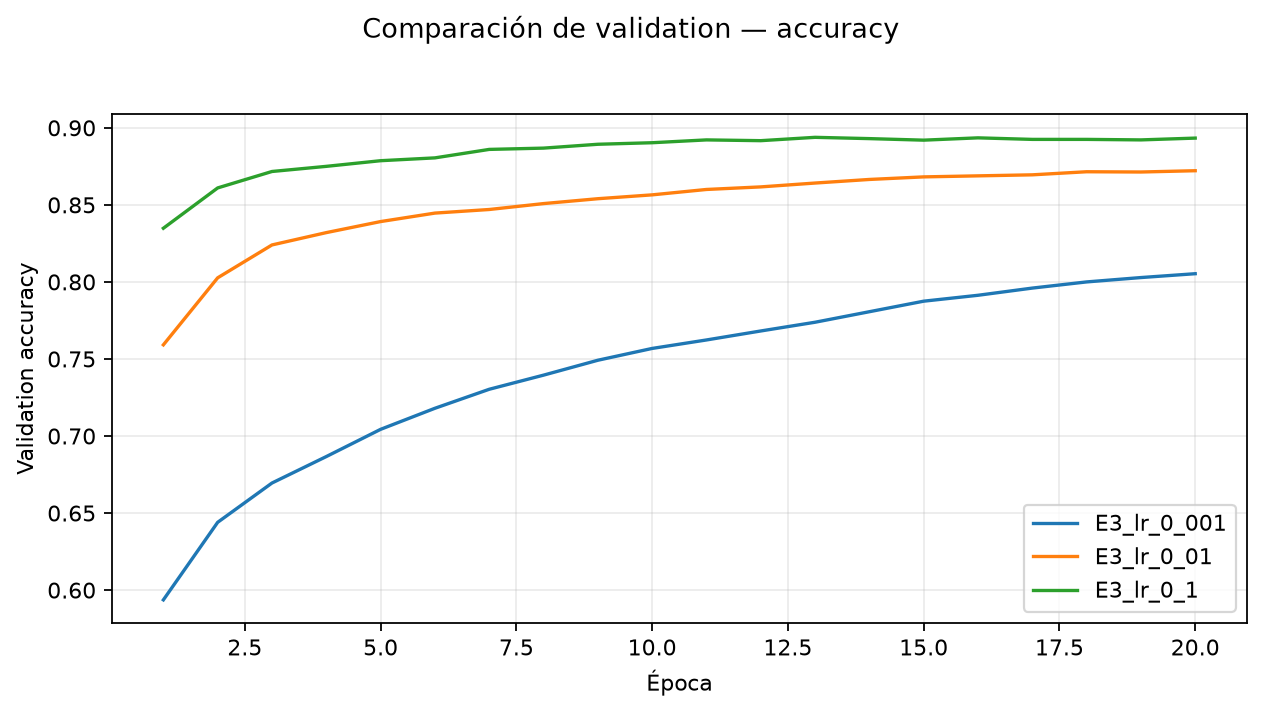
\includegraphics[width=\linewidth]{../../../../results/figures/E3_learning_rate_validation_accuracy.png}
\end{minipage}
\begin{minipage}{0.49\textwidth}
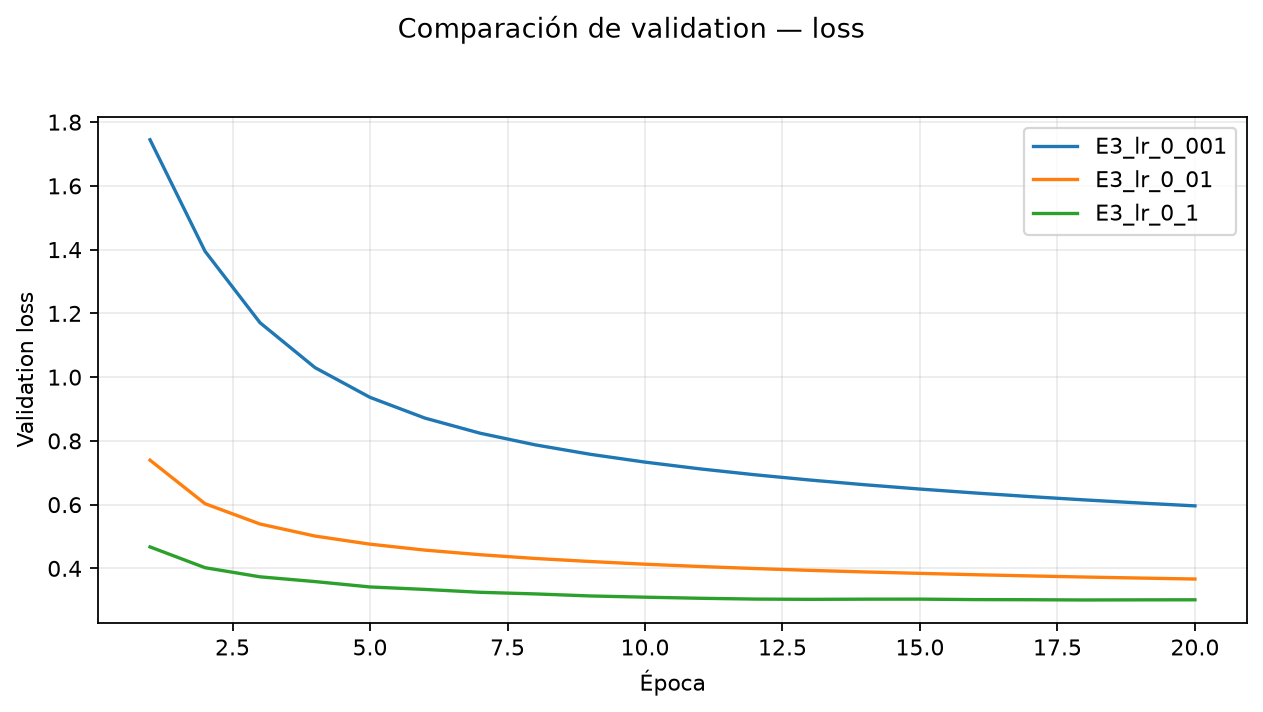
\includegraphics[width=\linewidth]{../../../../results/figures/E3_learning_rate_validation_loss.png}
\end{minipage}
\caption{Curvas de validation para E3.}
\end{figure}

\section{E4: tamaño de batch}

\begin{table}[H]
\centering
\begin{tabular}{lrrrr}
\toprule
Batch & Accuracy & F1 Macro & Gap loss & Duración ref. (s) \\
\midrule
32  & 0,8860 & 0,8864 & 0,2022 & 57,46 \\
128 & \textbf{0,8933} & \textbf{0,8936} & 0,0885 & 20,98 \\
512 & 0,8745 & 0,8771 & \textbf{0,0303} & \textbf{10,01} \\
\bottomrule
\end{tabular}
\caption{Comparación controlada de batch size sobre validation.}
\end{table}

Batch 128 obtuvo la mayor Accuracy y F1 Macro con costo intermedio. Batch 32 fue más lento y mostró deterioro posterior a sus mejores épocas. Batch 512 fue el más eficiente y presentó gaps menores, pero perdió 1,88 puntos porcentuales de Accuracy frente a 128. Por ello, batch 128 se mantuvo como control para E5.

\begin{figure}[H]
\centering
\begin{minipage}{0.49\textwidth}
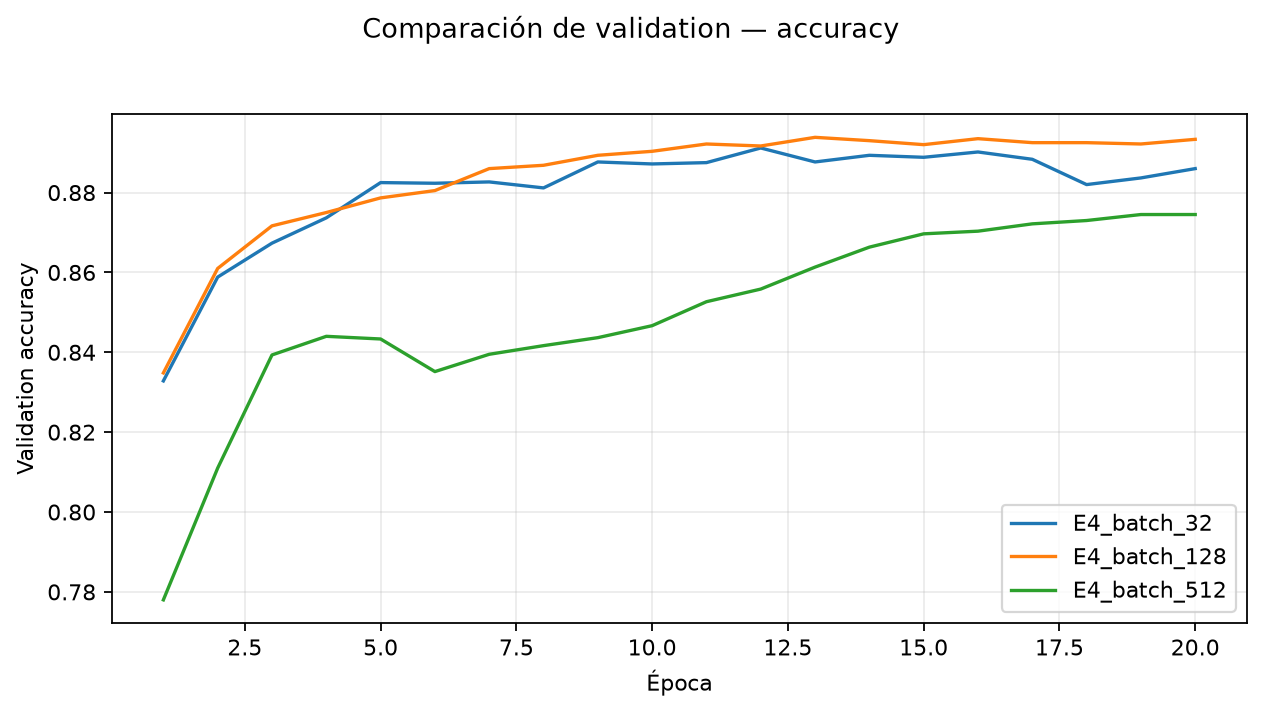
\includegraphics[width=\linewidth]{../../../../results/figures/E4_batch_size_validation_accuracy.png}
\end{minipage}
\begin{minipage}{0.49\textwidth}
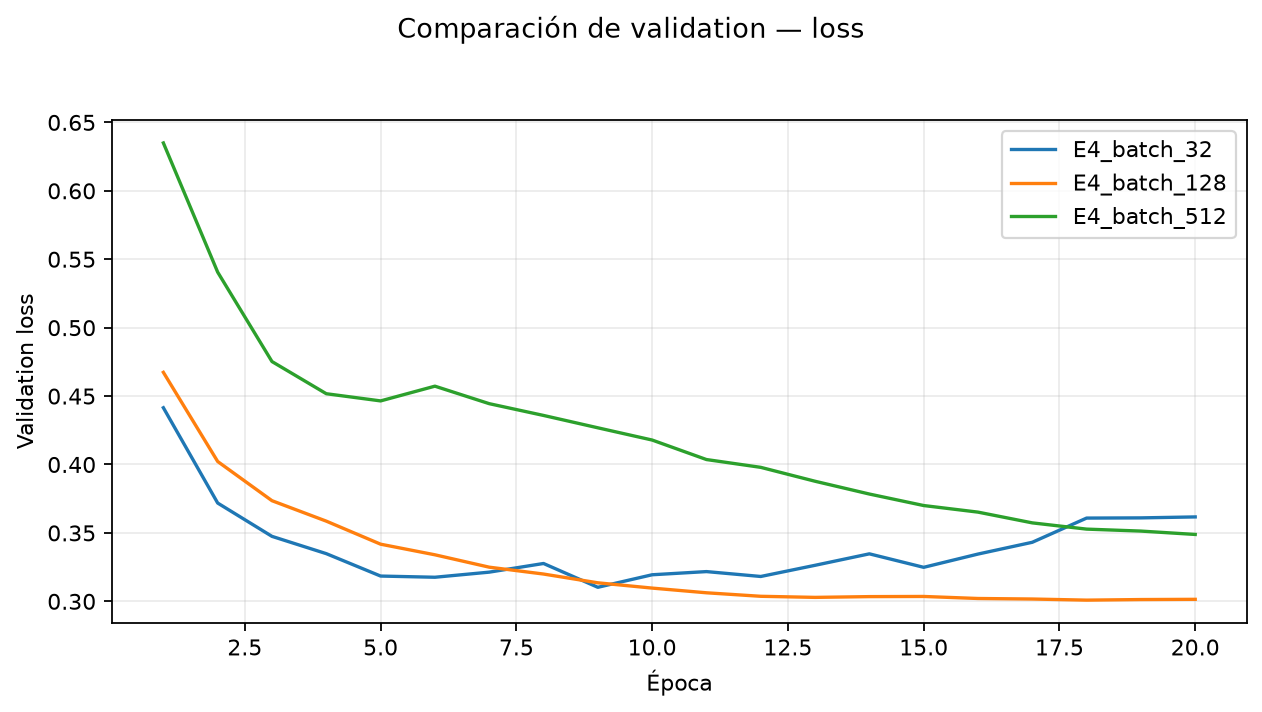
\includegraphics[width=\linewidth]{../../../../results/figures/E4_batch_size_validation_loss.png}
\end{minipage}
\caption{Curvas de validation para E4.}
\end{figure}

\section{E5: capacidad de la MLP}

\begin{table}[H]
\centering
\begin{tabular}{lrrrrr}
\toprule
Capas ocultas & Parámetros & Accuracy & F1 Macro & Gap loss & Duración ref. (s) \\
\midrule
$[64]$ & 50.890 & 0,8873 & 0,8881 & \textbf{0,0256} & \textbf{12,09} \\
$[256,128]$ & 235.146 & 0,8933 & 0,8936 & 0,0885 & 19,52 \\
$[512,256,128]$ & 567.434 & \textbf{0,8990} & \textbf{0,8989} & 0,1215 & 31,32 \\
\bottomrule
\end{tabular}
\caption{Comparación controlada de capacidad sobre validation.}
\end{table}

La red grande obtuvo el mayor desempeño absoluto, pero su mejora frente a $[256,128]$ fue de 0,57 puntos porcentuales de Accuracy y 0,53 de F1 Macro, a cambio de 2,41 veces más parámetros y gaps mayores. En la corrida de referencia también tardó 1,60 veces más; esta proporción temporal puede variar y no se usa como criterio aislado.

Se seleccionó $[256,128]$ como candidata equilibrada. Esta elección conserva una alternativa compacta, $[64]$, y una alternativa orientada a desempeño absoluto, $[512,256,128]$, sin presentar la candidata como arquitectura definitiva.

\begin{figure}[H]
\centering
\begin{minipage}{0.49\textwidth}
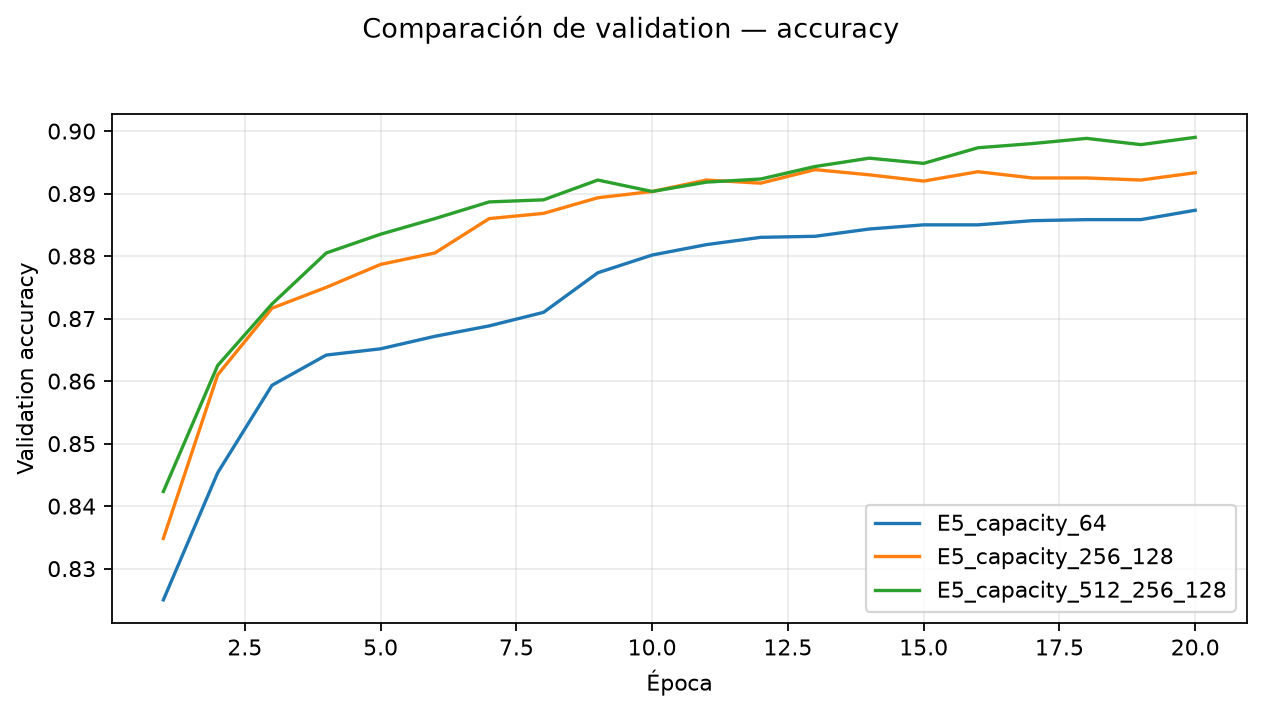
\includegraphics[width=\linewidth]{../../../../results/figures/E5_capacity_validation_accuracy.png}
\end{minipage}
\begin{minipage}{0.49\textwidth}
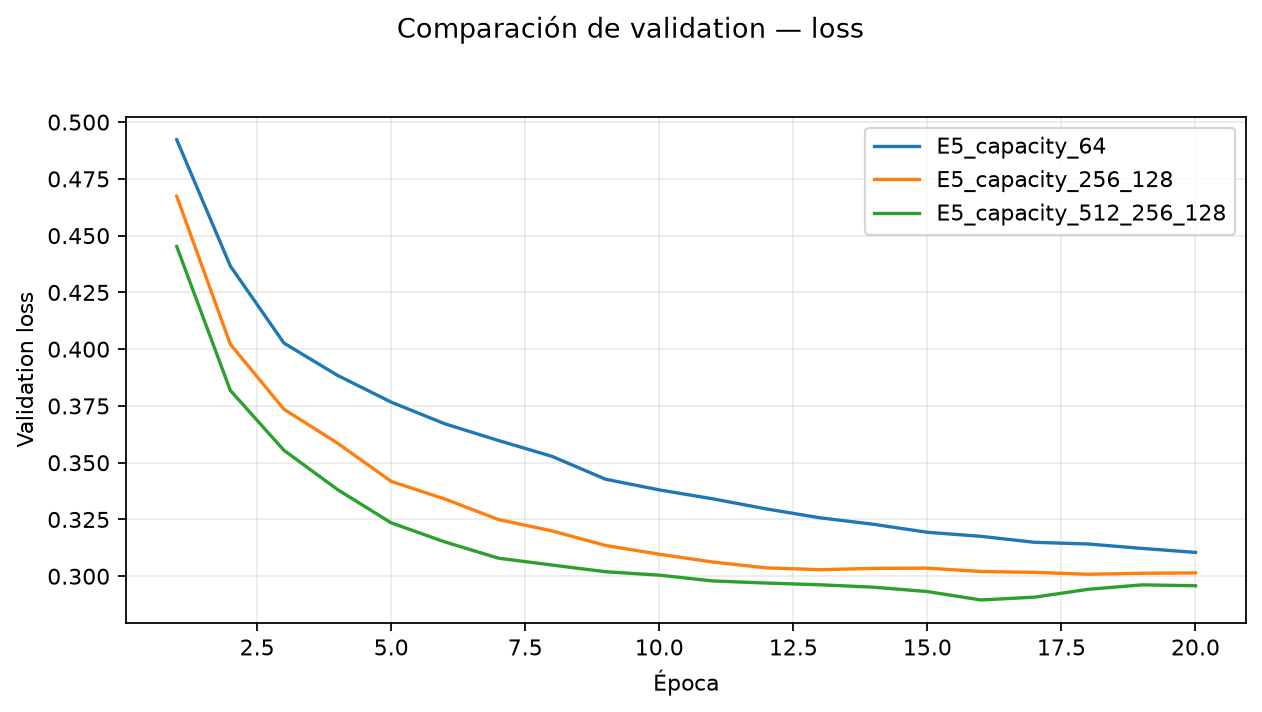
\includegraphics[width=\linewidth]{../../../../results/figures/E5_capacity_validation_loss.png}
\end{minipage}
\caption{Curvas de validation para E5.}
\end{figure}

\section{Métricas de la candidata}

\begin{table}[H]
\centering
\begin{tabular}{lr}
\toprule
Métrica de validation & Resultado \\
\midrule
Accuracy & 0,8933 \\
Precision Macro & 0,8949 \\
Recall Macro & 0,8933 \\
F1 Macro & 0,8936 \\
Precision ponderada & 0,8949 \\
Recall ponderado & 0,8933 \\
F1 ponderado & 0,8936 \\
\bottomrule
\end{tabular}
\caption{Métricas de la configuración candidata $[256,128]$.}
\end{table}

Validation contiene 600 ejemplos por clase. Debido a ese balance, las métricas macro y ponderadas coinciden en esta etapa; ambas se conservan para mantener un contrato explícito y permitir comparaciones futuras si cambia la distribución.

\section{Decisión sobre Early Stopping}

No se añadió un experimento con callback. Para la candidata, la menor validation loss fue 0,3009 en la época 18 y la final 0,3015; la diferencia aproximada de 0,0006 no representa un deterioro material y el ahorro potencial era de dos épocas. El ejecutor rechaza explícitamente \texttt{early\_stopping=true} mientras el callback no esté implementado, evitando registrar una técnica inexistente. La decisión debe reevaluarse si un nuevo optimizador o regularización cambia las curvas.

\section{Reproducibilidad, limitaciones y handoff}

La etapa se ejecutó dentro de \texttt{.venv} administrado por \texttt{uv}, con Python 3.12.x y dependencias bloqueadas en \texttt{uv.lock}. Las 22 pruebas automatizadas y Ruff 0.16.8 pasan. El notebook \path{notebooks/02_lucas_hyperparameters.ipynb} contiene seis celdas de código ejecutadas y cero errores.

Las comparaciones usan una seed. Las diferencias marginales requieren repetición antes de congelar el modelo final. Cesar recibe $[256,128]$, SGD, learning rate 0,1, batch 128 y 20 épocas como control para comparar optimizadores y regularización. Solo después de congelar la configuración y el protocolo podrá evaluarse una vez el test oficial.

\end{document}
